\section{Stepfile Difficulty Model}
\label{sec:stepfile_difficulty}

Stepfile difficulty has been a persistent subject of debate within the Flash Flash Revolution (FFR) community. Accurately defining the difficulty level of a specific sequence of keystrokes necessitates careful analysis of shared patterns across various stepfiles, which inherently exposes the process to player subjectivity. Despite attempts to leverage machine learning and artificial intelligence to address this issue, no solutions have successfully integrated the established concepts of stepfile difficulty. This limitation stems primarily from the fact that individual players possess diverse interpretations of what constitutes a difficult stepfile, shaped by their unique playing objectives and physical capabilities. Consequently, community resolutions regarding stepfile difficulty frequently result in biased judgments and disagreements. To effectively address these challenges, it is essential to standardize the definition of stepfile difficulty and to differentiate between the associated objective characteristics and the inherent subjectivity involved in such assessments.

\subsection{Playing Objective Categorizations}

\textit{Playing objectives} are goals players set to optimize in their gameplay. These playing objectives can be categorized into two main groups: constant weighted and variable weighted. This section focuses on providing numerous examples of both types of playing objectives, discussing their integration into our analysis, and establishing a default playing objective to be utilized in this report. It is imperative to acknowledge that, at present, ACubed currently supports only stepfile difficulty measurements under discretized constant weighted playing objectives. In upcoming releases, ACubed is expected to expand its capabilities to encompass additional playing objectives as we deliberate on methods to implement this in our framework.

\subsubsection{Constant-Weighted Playing Objectives}

A fundamental aspect of \textit{constant-weighted} playing objectives is the assumption that the reward for successfully hitting a note remains consistent at the note-level. Namely, each attempt at hitting a note in the stepfile receives a consistently defined reward value between $0$ and $1$, which reflects the player's incentive to successfully hit the note at some timestamp relative to the exact timing requirements for a given note. The following are examples of commonly used playing objectives falling within this category.

\begin{itemize}
    \item The Full-Combo (FC) score incentivizes players to hit all notes without missing any. The reward function to FC a stepfile is:

    $$r(t) = \begin{cases} 
          1 & -117 \leq t \leq 118 \\
          0 & \text{otherwise}
       \end{cases}$$

    \item To achieve a Clean Full-Combo score, players must hit all notes without any average hits or boo hits in addition to achieving an FC on the stepfile. The reward function to Clean FC a stepfile is:

    $$r(t) = \begin{cases} 
          1 & -83 \leq t \leq 118 \\
          0 & \text{otherwise}
       \end{cases}$$

    \item In order to maximize the score under FFR's Judge Windows, players should aim to optimize the raw score of a stepfile using the specified weights discussed in the previous section. The reward function to maximize raw score under FFR scoring is:

    $$r(t) = \begin{cases} 
          0.1 & -117 \leq t < -83 \\
          0.5 & -83 \leq t < -50 \\
          1 & -50 \leq t \leq 50 \\
          0.5 & 50 < t \leq 118 \\
          0 & \text{otherwise}
       \end{cases}$$

    \item Maximizing the score under MS Timing is not specific to FFR, but it involves optimizing the raw score of a stepfile where the assigned rewards favor hits that are closest to Perfect. This method of scoring is commonly implemented in other rhythm games, such as Etterna. The reward function to maximize raw score under MS timing is:

    $$r(t) = \begin{cases} 
          1- \frac{t}{118} & 0 \leq t \leq 118 \\
          1 + \frac{t}{117} & -117 \leq t \leq 0 \\
          0 & \text{otherwise}
       \end{cases}$$

    \item Scoring a AAA on a stepfile requires players to hit all notes within FFR's Perfect timing window. AAA is the maximum score a player can obtain on any stepfile in FFR. The reward function to score a AAA on a stepfile is:

    $$r(t) = \begin{cases} 
          1 & -50 \leq t \leq 50 \\
          0 & \text{otherwise}
       \end{cases}$$

    \item Scoring a AAAA on a stepfile requires players to hit all notes within FFR's Marvelous timing window. Despite AAAA's being significantly more difficult to obtain, these scores are treated as AAA for ranking purposes. The reward function to score a AAAA on a stepfile is:

    $$r(t) = \begin{cases} 
          1 & -17 \leq t \leq 17 \\
          0 & \text{otherwise}
       \end{cases}$$
\end{itemize}

Figure \ref{fig:playing_objectives} visually presents the various playing objectives, with the green colors denoting the reward given when a player successfully hits the correct note within the predetermined judge window.  

\begin{figure}[H]
\centering
\begin{tikzpicture}

    \begin{scope}
        \shade[top color=perfect-color, bottom color=perfect-color] (-1,-1) rectangle (4,0);
\shade[top color=perfect-color, bottom color=perfect-color] (-1,0) rectangle (4,1);
\node[inner sep=0pt] (left) at (0,0)
    {
\includegraphics[width=1cm]{figures/receptor/left.png}};
\node[inner sep=0pt] (down) at (1,0)
    {
\includegraphics[width=1cm]{figures/receptor/down.png}};
\node[inner sep=0pt] (up) at (2,0)
    {
\includegraphics[width=1cm]{figures/receptor/up.png}};
\node[inner sep=0pt] (right) at (3,0)
    {
\includegraphics[width=1cm]{figures/receptor/right.png}};
\node[inner sep=0pt] at (-1,-1)[label=left:{\footnotesize\texttt{118ms}}]{};
\draw[opacity=0.5,dashed] (-1, -1) -- (4, -1); 
\node[inner sep=0pt] at (-1,0) [label=left:{\footnotesize \texttt{0ms}}]{};
\draw[opacity=0.5,dashed] (-1, 0) -- (4, 0); 
\node[inner sep=0pt] at (-1,1) [label=left:{\footnotesize \texttt{-117ms}}]{};
\draw[opacity=0.5,dashed] (-1, 1) -- (4, 1);
\node[inner sep=0pt] at (1.5, -1.5) [label=center:{\footnotesize \textit{(a)} Full-Combo (FC)}]{};
    \end{scope}

    \begin{scope}[xshift=8cm]
\shade[top color=perfect-color, bottom color=perfect-color] (-1,-1) rectangle (4,0);
\shade[top color=perfect-color, bottom color=perfect-color] (-1,0) rectangle (4,0.083/0.118);
\node[inner sep=0pt] (left) at (0,0)
    {
\includegraphics[width=1cm]{figures/receptor/left.png}};
\node[inner sep=0pt] (down) at (1,0)
    {
\includegraphics[width=1cm]{figures/receptor/down.png}};
\node[inner sep=0pt] (up) at (2,0)
    {
\includegraphics[width=1cm]{figures/receptor/up.png}};
\node[inner sep=0pt] (right) at (3,0)
    {
\includegraphics[width=1cm]{figures/receptor/right.png}};
\node[inner sep=0pt] at (-1,-1)[label=left:{\footnotesize\texttt{118ms}}]{};
\draw[opacity=0.5,dashed] (-1, -1) -- (4, -1); 
\node[inner sep=0pt] at (-1,0) [label=left:{\footnotesize \texttt{0ms}}]{};
\draw[opacity=0.5,dashed] (-1, 0) -- (4, 0); 
\node[inner sep=0pt] at (-1,1) [label=left:{\footnotesize \texttt{-117ms}}]{};
\draw[opacity=0.5,dashed] (-1, 1) -- (4, 1);
\node[inner sep=0pt] at (1.5, -1.5) [label=center:{\footnotesize \textit{(b)} Clean Full-Combo (FC)}]{};
    \end{scope}

    \begin{scope}[yshift=-3.5cm]
        \shade[top color=perfect-color, bottom color=perfect-color, opacity=0.5] (-1,-1) rectangle (4,-0.050/0.117);
\shade[top color=perfect-color, bottom color=perfect-color] (-1,-0.050/0.117) rectangle (4,0);
\shade[top color=perfect-color, bottom color=perfect-color] (-1,0) rectangle (4,0.050/0.118);
\shade[top color=perfect-color, bottom color=perfect-color, opacity=0.5] (-1,0.050/0.118) rectangle (4,0.083/0.118);
\shade[top color=perfect-color, bottom color=perfect-color, opacity=0.1] (-1,0.083/0.118) rectangle (4,1);
\node[inner sep=0pt] (left) at (0,0)
    {
\includegraphics[width=1cm]{figures/receptor/left.png}};
\node[inner sep=0pt] (down) at (1,0)
    {
\includegraphics[width=1cm]{figures/receptor/down.png}};
\node[inner sep=0pt] (up) at (2,0)
    {
\includegraphics[width=1cm]{figures/receptor/up.png}};
\node[inner sep=0pt] (right) at (3,0)
    {
\includegraphics[width=1cm]{figures/receptor/right.png}};
\node[inner sep=0pt] at (-1,-1)[label=left:{\footnotesize\texttt{118ms}}]{};
\draw[opacity=0.5,dashed] (-1, -1) -- (4, -1); 
\node[inner sep=0pt] at (-1,0) [label=left:{\footnotesize \texttt{0ms}}]{};
\draw[opacity=0.5,dashed] (-1, 0) -- (4, 0); 
\node[inner sep=0pt] at (-1,1) [label=left:{\footnotesize \texttt{-117ms}}]{};
\draw[opacity=0.5,dashed] (-1, 1) -- (4, 1);
\node[inner sep=0pt] at (1.5, -1.5) [label=center:{\footnotesize \textit{(c)} Maximize Score under FFR Scoring (Default)}]{};
    \end{scope}

    \begin{scope}[xshift=8cm, yshift=-3.5cm]
\shade[top color=perfect-color, bottom color=white] (-1,-1) rectangle (4,0);
\shade[top color=white, bottom color=perfect-color] (-1,0) rectangle (4,1);
\node[inner sep=0pt] (left) at (0,0)
    {
\includegraphics[width=1cm]{figures/receptor/left.png}};
\node[inner sep=0pt] (down) at (1,0)
    {
\includegraphics[width=1cm]{figures/receptor/down.png}};
\node[inner sep=0pt] (up) at (2,0)
    {
\includegraphics[width=1cm]{figures/receptor/up.png}};
\node[inner sep=0pt] (right) at (3,0)
    {
\includegraphics[width=1cm]{figures/receptor/right.png}};
\node[inner sep=0pt] at (-1,-1)[label=left:{\footnotesize\texttt{118ms}}]{};
\draw[opacity=0.5,dashed] (-1, -1) -- (4, -1); 
\node[inner sep=0pt] at (-1,0) [label=left:{\footnotesize\texttt{0ms}}]{};
\draw[opacity=0.5,dashed] (-1, 0) -- (4, 0); 
\node[inner sep=0pt] at (-1,1) [label=left:{\footnotesize\texttt{-117ms}}]{};
\draw[opacity=0.5,dashed] (-1, 1) -- (4, 1);
\node[inner sep=0pt] at (1.5, -1.5) [label=center:{\footnotesize \textit{(d)} Maximize Score under MS-based Timings}]{};
    \end{scope}

    \begin{scope}[yshift=-7cm]
\shade[top color=perfect-color, bottom color=perfect-color] (-1,-0.050/0.117) rectangle (4,0.050/0.118);
\node[inner sep=0pt] (left) at (0,0)
    {
\includegraphics[width=1cm]{figures/receptor/left.png}};
\node[inner sep=0pt] (down) at (1,0)
    {
\includegraphics[width=1cm]{figures/receptor/down.png}};
\node[inner sep=0pt] (up) at (2,0)
    {
\includegraphics[width=1cm]{figures/receptor/up.png}};
\node[inner sep=0pt] (right) at (3,0)
    {
\includegraphics[width=1cm]{figures/receptor/right.png}};
\node[inner sep=0pt] at (-1,-1)[label=left:{\footnotesize\texttt{118ms}}]{};
\draw[opacity=0.5,dashed] (-1, -1) -- (4, -1); 
\node[inner sep=0pt] at (-1,0) [label=left:{\footnotesize \texttt{0ms}}]{};
\draw[opacity=0.5,dashed] (-1, 0) -- (4, 0); 
\node[inner sep=0pt] at (-1,1) [label=left:{\footnotesize \texttt{-117ms}}]{};
\draw[opacity=0.5,dashed] (-1, 1) -- (4, 1);
\node[inner sep=0pt] at (1.5, -1.5) [label=center:{\footnotesize \textit{(e)} All Perfects (AAA)}]{};
    \end{scope}

    \begin{scope}[xshift=8cm, yshift=-7cm]
\shade[top color=perfect-color, bottom color=perfect-color] (-1,-0.017/0.117) rectangle (4,0.017/0.118);
\node[inner sep=0pt] (left) at (0,0)
    {
\includegraphics[width=1cm]{figures/receptor/left.png}};
\node[inner sep=0pt] (down) at (1,0)
    {
\includegraphics[width=1cm]{figures/receptor/down.png}};
\node[inner sep=0pt] (up) at (2,0)
    {
\includegraphics[width=1cm]{figures/receptor/up.png}};
\node[inner sep=0pt] (right) at (3,0)
    {
\includegraphics[width=1cm]{figures/receptor/right.png}};
\node[inner sep=0pt] at (-1,-1)[label=left:{\footnotesize\texttt{118ms}}]{};
\draw[opacity=0.5,dashed] (-1, -1) -- (4, -1); 
\node[inner sep=0pt] at (-1,0) [label=left:{\footnotesize \texttt{0ms}}]{};
\draw[opacity=0.5,dashed] (-1, 0) -- (4, 0); 
\node[inner sep=0pt] at (-1,1) [label=left:{\footnotesize \texttt{-117ms}}]{};
\draw[opacity=0.5,dashed] (-1, 1) -- (4, 1);
\node[inner sep=0pt] at (1.5, -1.5) [label=center:{\footnotesize \textit{(f)} All Marvelous (AAAA)}]{};
    \end{scope}

\end{tikzpicture}

\caption{Constant-Weighted Playing Objectives to define Stepfile Difficulty.} \label{fig:playing_objectives}
\end{figure}

It is worth mentioning that since the manually assigned difficulty ratings are determined under the goal of achieving the highest possible raw score with FFR judgement windows, our definition of the stepfile difficulty model will be aligned with this particular playing objective. Additional manual data collection is necessary to develop a stepfile difficulty model that can support other playing objectives identified in this report.

\vspace{2mm}

To allow for meaningful comparisons, each playing objective can be represented by an equivalent judge window size $J$. This can be determined by evaluating the following integral:

$$J = \displaystyle \int_{-\infty}^{\infty} r(t) dt$$

For example, for score maximizing playing objectives under FFR judgement windows, we have:
\begin{align*}
J &= \displaystyle \int_{-\infty}^{\infty} r(t) dt \\
& = 0.1 \cdot (-83 - (-117)) + 0.5 \cdot (-50 - (-83)) + 1 \cdot (50 - (-50)) + 0.5 \cdot (118 - 50) \\
&= 3.4 + 16.5 + 100 + 34 = 153.9
\end{align*}

and for score maximizing playing objectives under MS Timing, we have:
\begin{align*}
J &= \displaystyle \int_{-\infty}^{\infty} r(t) dt \\
& = \int_{0}^{118} \left(1 - \frac{t}{118}\right) dt + \int_{-117}^{0} \left(1 + \frac{t}{117}\right) dt \\
&= \left. \left( t - \frac{t^2}{236} \right)\right|_{t = 118} - \left.\left( t + \frac{t^2}{234} \right) \right|_{t = - 117} \\
&= 59 + 58.5 = 117.5
\end{align*}

Moreover, with the assumption that the weight values for Etterna's Perfect, Great, and Good ratings are $1$, $0.5$, and $0.1$ respectively, \href{https://docs.google.com/spreadsheets/d/1syi5aN6sTiDA2Bs_lzZjsLQ1yCEhxl5EnAd6EsD6cF4/edit?gid=0#gid=0}{Etterna Judgement Data} was incorporated into the analysis for comparison. Through similar calculations, it was determined that the corresponding equivalent judge window sizes for each identified playing objective are as follows:

\begin{center}
	\begin{tabular}{c@{\hskip 5mm}c}
		\hspace{5mm} \textbf{Playing Objective} \hspace{5mm} & \textbf{Equivalent Window Size} $J$ \\
            \hline
		Full-Combo in FFR                              & 235                        \\
            Maximize Score in Etterna Under J1 & 216\\
		Clean Full-Combo in FFR                                 & 201                         \\
            Maximize Score in Etterna Under J2 & 191.52\\
            Maximize Score in Etterna Under J3 & 167.04\\
		Maximize Score in FFR assuming default scoring                              & 153.9                       \\
            Maximize Score in Etterna Under J4 & 144\\
            Maximize Score in Etterna Under J5 & 120.96\\
		Maximize Score in FFR assuming MS-weighted scoring                                  & 117.5                       \\
  
		Scoring AAA in FFR                                   & 100                    \\
            Maximize Score in Etterna Under J6 & 95.04\\
            Maximize Score in Etterna Under J7 & 72\\
            Maximize Score in Etterna Under J8 & 47.52\\
		Scoring AAAA in FFR                                   & 34                       \\
            Maximize Score in Etterna Under J9 & 28.8\\
	\end{tabular}
\end{center}

The execution of the playing objective is more challenging when $J$ values are lower, as indicated by a smaller judge window which allows for a narrower margin of error. This examination corroborates the general perception within the community that the FFR's scoring system falls between Etterna's J3 and J4 scoring, with the latter being known as Etterna's default judgement setting. 

\vspace{2mm}

These computed judge windows will be utilized in this report to enhance the definition of objective features that are employed in the stepfile difficulty model. Further details on integrating judge window size to the objective features associated to the stepfile difficulty model will be discussed later in this section.

\subsubsection{Variable-Weighted Playing Objectives}

The concept of variable-weighted playing objectives posits that the reward attributed to each note can vary depending on the player's previous actions. This means that the reward value, which similarly ranges from 0 to 1, does not necessarily require a perfect hit for every note to fulfill the playing objective. The following playing objectives are categorized as variable-weighted:

\begin{itemize}
    \item The utilization of atypical playing tactics for the purpose of generating non-conventional scores is a fundamental aspect of the Anti-PA scoring methodology. This strategic approach is typically employed by players in order to unlock \href{https://www.flashflashrevolution.com/tokens/skill_token_info.php}{skill tokens in FFR}.

    \item In order to obtain a Single-Digit Good (SDG) score, players must achieve a score of less than ten raw goods on a stepfile. SDG is commonly recognized by players as a crucial milestone in their pursuit of achieving a AAA score on that particular stepfile.
\end{itemize}



It is worth noting that the aforementioned examples can be generalized as scoring-based objectives, in which the player's aim is to reach a predetermined score. However, depending on the miss and boo requirements of the targeted score, the player must additionally manage the life bar when gameplay is in session. Shown on the right of Figure \ref{fig:gameplay}, the life bar represents a player's remaining life during gameplay. Each successful hit on an arrow contributes to increasing the bar, whereas receiving a Miss or Boo judgement will result in a decrease. Allowing the bar to deplete entirely will result in the conclusion of the game.

\begin{center}
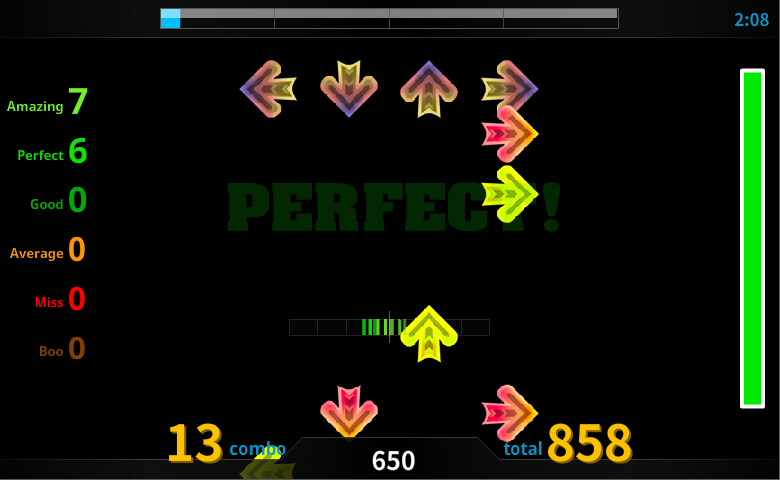
\includegraphics[width=10cm]{figures/images/gameplay.png}
\captionof{figure}{Screenshot of FFR's Gameplay View (upscroll view)}
\label{fig:gameplay}
\end{center}

While the addition of the life bar in gameplay introduces implementation challenges in measuring the difficulty of these playing objectives, we offer potential solutions for addressing this issue. We commence by positing a theorem and reinforcing it with a heuristic demonstration.

\begin{theorem}
\label{thm:finiteness}
Given any targeted score under the variable-weighted playing objective, there are finitely many ways for a player to accomplish this. 
\end{theorem}

\begin{proof}
    Let $B$ represent the number of boos in the targeted score and let $N$ represent the number of notes in the stepfile. As boos can only appear between two notes, we can count the number of ways to assort $B$ boos with $N$ notes using stars and bars. Let $\times$ represent boos and $\mid$ represent notes, and arrange the objects sequentially as shown in Figure \ref{fig:starsandbars1}.

\vspace{2mm}

\begin{center}
$ \times \mid\times\mid \; \mid \times \times \mid \; \mid \; \mid \times$
\captionof{figure}{An example of Stars and Bars for $N=6$ notes and $B =5$ boos}
\label{fig:starsandbars1}
\end{center}

Because there are a total of $N+B$ objects, there are $\displaystyle \binom{N+B}{B}$ ways to arrange $N$ notes and $B$ boos.

\vspace{2mm}

Furthermore, let $H$ represent the number of successfully hit notes and $M$ represent the number of missed notes. Observe that $H + M = N$. Using the previously discussed Stars and Bars analogy, if we let $+$ and $-$ represent hits and misses respectively while ignoring the $\times$, we can replace each $\mid$ with these symbols as shown in Figure \ref{fig:starsandbars2}.

\vspace{2mm}

Per arrangement from the first iteration of Stars and Bars, there are $\displaystyle\binom{H + M}{M}$ ways to arrange $H$ hits and $M$ misses.

\begin{center}
$ \times \mid\times\mid \; \mid \times \times \mid \; \mid \; \mid \times$ 	\hspace{5mm} $\Longrightarrow$ \hspace{5mm} $\times + \times +  - \times \times ++- \times $
\captionof{figure}{Replacing $N=6$ notes with $H=4$ hits and $M = 2$ misses}
\label{fig:starsandbars2}
\end{center}

We apply the same argument to conclude that the number of ways to arrange $P$ perfects, $G$ goods, and $A$ averages over $H = P + G + A$ hits is:
$$\displaystyle \binom{P + G + A}{A}\binom{P+G}{G}$$

Combining everything together, the number of possible ways a player can score $P$ perfects, $G$ goods, $A$ averages, $M$ misses, and $B$ boos in a stepfile containing $N$ notes, regardless of the life bar's status, is:
$$\displaystyle \binom{P+G+A+M+B}{B}\binom{P+G+A+M}{M} \binom{P + G + A}{A}\binom{P+G}{G} = \binom{N+B}{P, G, A, M, B}.$$

We can obtain sharper upper bounds when we consider the status of the life bar in our overall counts. Using the same variable definitions, let $J$ represent the number of ``no-hit" actions (i.e. $J = M + B$). Then, our combinatorics problem can be reformulated as:
$$j_1 + j_2 + \cdots + j_{H + 1} = H + J$$

where $j_i$ represents the number of ``no-hit" actions in the $i$th bin (i.e. number of misses and boos between the $(i-1)$th and $i$th hits). Applying Stars and Bars without any constraints, the number of integer solutions to the above problem is $\displaystyle \binom{H+J}{H}$.

\vspace{2mm}

As the maximum health in the life bar is $20$, then for all $j_i$, we have $j_i \leq 20$. To enforce the constraint for $k$ $j_i$'s, we need to exclude all solutions with $j_{i_1} > 20$, $j_{i_2} > 20$, $\cdots$, $j_{i_k} > 20$ for $0 \leq i_1 \neq i_2 \neq \cdots \neq i_k \leq \left\lfloor\frac{J}{21} \right\rfloor$ (to ensure that $J - 21k \geq 0$). The above problem under these constraints can be reformulated as:
$$j_1 + \cdots + (j_{i_1} - 21) + (j_{i_2} - 21) + \cdots + (j_{i_k} - 21) 
+ \cdots + j_{H + 1} = H + J - 21k.$$

There are $\displaystyle \binom{H+1}{k}$ ways to choose the $k$ $j_i$'s and for each $k$, there are $\displaystyle\binom{H+J-21k}{H}$ solutions.

\vspace{2mm}

By applying the Inclusion–Exclusion principle across all $k-$tuples of $j_i$'s satisfying the above constraint, we get:
$$\sum_{k =0}^{\left\lfloor \frac{J}{21}\right\rfloor} (-1)^k \binom{H + 1}{k}\binom{H+J-21k}{H}.$$

Therefore, the number of possible ways a player can score $P$ perfects, $G$ goods, $A$ averages, $M$ misses, and $B$ boos in a stepfile containing $N$ notes is:
$$\sum_{k =0}^{\left\lfloor \frac{M+B}{21}\right\rfloor} (-1)^k \binom{P+G+A + 1}{k}\binom{N+B-21k}{P+G+A}.$$

We claim that this count is an upper bound to the total number of ways a player can actually produce such scores in actual gameplay. This is due to the fact that the count accounts for scenarios where $j_1 \geq 10$ (indicating that the number of misses and boos before hitting the first note is greater than or equal to $10$) is not deemed a failure, when in reality it would result in the conclusion of the game. 

\end{proof}

Let $f$ represent the stepfile difficulty model that maps the set of all input configurations that result in a predetermined desired score $\mathcal{C}_{\text{score}}$ to a positive real number. Hence, following the establishment of finiteness through Theorem \ref{thm:finiteness}, it can be deduced that there exists an input configuration such that $f$ is minimal. This particular configuration can be considered as the most optimal way for a player to achieve the desired score.

\vspace{2mm}

It is assumed that if a player is able to achieve a higher-rated input configuration, then they are also capable of achieving the optimal configuration. Under this assumption, we rate the stepfile difficulty under variable-weighted playing objectives by evaluating the following optimization problem:

\begin{equation*}
\begin{aligned}
\min_{c \in \mathcal{C}_{\text{score}}} \quad & f(c)\\
\textrm{s.t.} \quad & \text{score} = (P, G, A, M, B)  
\end{aligned}
\end{equation*}

Currently, the exact criteria for determining the judge window size in variable-weighted playing objectives has yet to be established. Without loss of generality, consider all notes in a given stepfile that are oriented upwards. We will refer to the example shown in Figure \ref{fig:boos} for context.

\begin{center}
\begin{tikzpicture}
        \shade[top color=perfect-color, bottom color=perfect-color, opacity=0.5] (-1,-1 +2.5+1.25) rectangle (4,-0.050/0.117 +2.5+1.25);
\shade[top color=perfect-color, bottom color=perfect-color] (-1,-0.050/0.117 +2.5+1.25) rectangle (4,0.050/0.118 +2.5+1.25);
\shade[top color=perfect-color, bottom color=perfect-color, opacity=0.5] (-1,0.050/0.118 +2.5+1.25) rectangle (4,0.083/0.118 +2.5+1.25);
\shade[top color=perfect-color, bottom color=perfect-color, opacity=0.1] (-1,0.083/0.118 +2.5+1.25) rectangle (4,1 +2.5+1.25);
\node[inner sep=0pt] (up) at (2,0 +2.5+1.25)
    {
\includegraphics[width=1cm]{figures/016/up.png}};



        \shade[top color=perfect-color, bottom color=perfect-color, opacity=0.5] (-1,-1 +2.5) rectangle (4,-0.050/0.117 +2.5);
\shade[top color=perfect-color, bottom color=perfect-color] (-1,-0.050/0.117 +2.5) rectangle (4,0.050/0.118 +2.5);
\shade[top color=perfect-color, bottom color=perfect-color, opacity=0.5] (-1,0.050/0.118 +2.5) rectangle (4,0.083/0.118 +2.5);
\shade[top color=perfect-color, bottom color=perfect-color, opacity=0.1] (-1,0.083/0.118 +2.5) rectangle (4,1 +2.5);
\node[inner sep=0pt] (up) at (2,0 +2.5)
    {
\includegraphics[width=1cm]{figures/008/up.png}};
        
        \shade[top color=perfect-color, bottom color=perfect-color, opacity=0.5] (-1,-1) rectangle (4,-0.050/0.117);
\shade[top color=perfect-color, bottom color=perfect-color] (-1,-0.050/0.117) rectangle (4,0.050/0.118);
\shade[top color=perfect-color, bottom color=perfect-color, opacity=0.5] (-1,0.050/0.118) rectangle (4,0.083/0.118);
\shade[top color=perfect-color, bottom color=perfect-color, opacity=0.1] (-1,0.083/0.118) rectangle (4,1);
\node[inner sep=0pt] (up) at (2,0)
    {
\includegraphics[width=1cm]{figures/004/up.png}};

\node[inner sep=0pt] (left) at (0,-1.75)
    {
\includegraphics[width=1cm]{figures/receptor/left.png}};
\node[inner sep=0pt] (down) at (1,-1.75)
    {
\includegraphics[width=1cm]{figures/receptor/down.png}};
\node[inner sep=0pt] (up) at (2,-1.75)
    {
\includegraphics[width=1cm]{figures/receptor/up.png}};
\node[inner sep=0pt] (right) at (3,-1.75)
    {
\includegraphics[width=1cm]{figures/receptor/right.png}};

\draw[opacity=0.5,dashed] (-1, 2.5+0.625) -- (4, 2.5+0.625); 
\node[inner sep=0pt] at (-1,2.5+0.625) [label=left:{\footnotesize $b_2$}]{};
\node[inner sep=0pt] (up) at (2,2.5+0.625)
    {$\textcolor{orange}{\boldsymbol{\times}}$};
\node[inner sep=0pt] (up) at (2,2.5+0.625+0.01)
    {$\textcolor{orange}{\boldsymbol{\times}}$};
\node[inner sep=0pt] (up) at (2,2.5+0.625-0.01)
    {$\textcolor{orange}{\boldsymbol{\times}}$};
\node[inner sep=0pt] (up) at (2+0.01,2.5+0.625)
    {$\textcolor{orange}{\boldsymbol{\times}}$};
\node[inner sep=0pt] (up) at (2-0.01,2.5+0.625)
    {$\textcolor{orange}{\boldsymbol{\times}}$};

\draw[opacity=0.5,dashed] (-1, 1.25) -- (4, 1.25); 
\node[inner sep=0pt] at (-1,1.25) [label=left:{\footnotesize $b_1$}]{};
\node[inner sep=0pt] (up) at (2,1.25)
    {$\textcolor{orange}{\boldsymbol{\times}}$};
\node[inner sep=0pt] (up) at (2,1.25+0.01)
    {$\textcolor{orange}{\boldsymbol{\times}}$};
\node[inner sep=0pt] (up) at (2,1.25-0.01)
    {$\textcolor{orange}{\boldsymbol{\times}}$};
\node[inner sep=0pt] (up) at (2+0.01,1.25)
    {$\textcolor{orange}{\boldsymbol{\times}}$};
\node[inner sep=0pt] (up) at (2-0.01,1.25)
    {$\textcolor{orange}{\boldsymbol{\times}}$};

\end{tikzpicture}
\captionof{figure}{Incorporating Boos in Judge Window Size computation}
\label{fig:boos}
\end{center}

In the event that a player taps the keyboard at timestamp $b_1$ between the red and blue notes, the engine will record a Boo towards the final score. This is due to the fact that the judge windows for these notes do not overlap, allowing the possibility for the player to hit a Boo. The corresponding judge window size for successfully hitting this Boo is visually represented by the white-colored distance between the two judgment windows.

\vspace{2mm}

Conversely, if a player submits input at timestamp $b_2$ between the blue and yellow notes, the engine will record an early good in the judge window of the yellow note if the blue note was not previously hit, or a late good in the blue note's judge window if it was successfully hit. Given that these windows overlap, there is no opportunity for the player to hit a Boo, resulting in a judge window size of $0$ for this instance.

\vspace{2mm}

In terms of misses, as no action is required on the player's behalf, no judge window sizes are factored in the calculation of the overall difficulty of the stepfile under this playing objective. Essentially, misses can be disregarded as the domain space of all possible configurations assumes that the player will not fail the level.

\vspace{2mm}

Due to the fact that all variable-weighted playing objectives solely focus on players hitting a certain number of notes with different judgments, rather than specifying the exact timing of when to hit them, the evaluation of stepfile difficulty can be determined by finding the optimal configuration that increases the likelihood of achieving the desired judgments. This involves identifying the optimum judge window sizes and computing the overall weighted average once the configuration has been identified.

\subsection{Machine Learning Problem Formulation}

With a clear distinction made between different interpretations of difficulty, our focus now shifts to formulating the measurement of stepfile difficulty as a machine learning problem using the chosen definition as the de facto standard. In this section, we will define key terms and present a theorem as the basis for our methodology.

\vspace{2mm}

Stepfile features have a significant impact on identifying the factors that contribute to the level's difficulty. Thus, it is essential to utilize these features in constructing a predictive model for estimating stepfile difficulty. These features fall under two distinct categories, namely, objective and subjective.

\begin{itemize}
    \item \textit{Objective stepfile features} refer to characteristics of a stepfile that contain rigid requirements independent of the player's skill level. These may include precise timing requirements for all arrows and the duration of the stepfile. Note that meta stepfile features are not considered objective, as the established definition to differentiate patterns from one another cannot be codified deterministically. 
    \item \textit{Subjective stepfile features} are defined as elements that are primarily centered on the execution of the stepfile and are subject to the player's individual skill level. These features may include factors related to a player's ability to execute the steps accurately, as well as their access to high-quality equipment. For instance, a player with greater stamina is likely to excel at longer stepfiles and may tend to underestimate its level of challenge as a result. 
\end{itemize}

Using these stepfile features, we propose the following theorem.

\begin{theorem}
Given a stepfile, the true difficulty rating can be estimated with a machine learning model using the objective stepfile features and the upper echelons of player telemetry.
\end{theorem}

\begin{proof}

Consider a scenario where there are $n$ players, denoted as $A_1, A_2,\ldots,A_n$, tasked with providing feedback on the difficulty of a given stepfile. Each player, $A_i$ for all $1 \leq i \leq n$, relies on the stepfile's distinct attributes and their own personal abilities to justify their assessment. Assuming that the difficulty of the stepfile is additive, we can represent this as the following equation:
$$\text{Diff}_{\text{obs}}^{(A_i)} = \text{Diff}_{\text{obj}}^{(A_i)} + \text{Diff}_{\text{sub}}^{(A_i)}.$$

Because each player $A_1, A_2, \cdots, A_n$ are exposed to the same step layout in a given stepfile, their unbiased assessments of difficulty are mutually shared. This can be mathematically expressed as follows:
$$\text{Diff}_{\text{obj}} \coloneq \text{Diff}_{\text{obj}}^{(A_1)} = \text{Diff}_{\text{obj}}^{(A_2)} = \cdots = \text{Diff}_{\text{obj}}^{(A_n)}.$$

Let $A = (A_1, \cdots, A_n)$ denote a community of $n$ players. By aggregating the individual difficulty assessments of all $n$ players, we can calculate the observed difficulty rating of a stepfile, taking into consideration the potential impact of community bias. By further refining the aforementioned equation, we arrive at the following equation:
$$\text{Diff}_{\text{obs}}^{(A)} = \text{Diff}_{\text{obj}} + \text{Diff}_{\text{sub}}^{(A)}.$$

In theory, by obtaining feedback from the entire population regarding the difficulty of a stepfile, with an unlimited sample (i.e. $n \rightarrow \infty$), it may be possible to establish an accurate measurement of difficulty that considers human limitations and reduces the influence of player subjectivity. Therefore, 
$$\lim_{n \rightarrow \infty} \text{Diff}_{\text{obs}}^{(A)} = \text{Diff}_{\text{true}}\mspace{50mu} \text{and} \mspace{50mu} \lim_{n \rightarrow \infty} \text{Diff}_{\text{sub}}^{(A)} = \text{Diff}_{\text{human}}$$

for some unknown constant $\text{Diff}_{\text{human}}$. Based on the aforementioned asymptotic analysis, it can be deduced that
$$\text{Diff}_{\text{true}} = \text{Diff}_{\text{obj}} + \text{Diff}_{\text{human}}.$$
\end{proof}

It should be noted that the current difficulty ratings in the game are represented by $\text{Diff}_{\text{obs}}^{(A)}$ in the preceding proof. Based on this, we introduce the following corollary:

\begin{corollary}
The discrepancy between the true difference $\text{Diff}_{\text{true}}$ and the observed difference $\text{Diff}_{\text{obs}}^{(A)}$ is significantly influenced by the subjective characteristics of the stepfile as defined by the vocal community. In other words,
$$|\text{Diff}_{\text{obs}}^{(A)} - \text{Diff}_{\text{true}}| = |\text{Diff}_{\text{sub}}^{(A)} - \text{Diff}_{\text{human}}|$$
\end{corollary}

In order to ensure the credibility of the given target values, it is crucial to minimize the deviation between $\text{Diff}_{\text{obs}}^{(A)}$ and $\text{Diff}_{\text{true}}$. From the above corollary, this can be accomplished by utilizing community feedback to estimate $\text{Diff}_{\text{human}}$, the role which difficulty consultants play when receiving new opinions from community members. This requires us to gather more feedback from the community, which is highly susceptible to self-selection bias and group attribution error.

\vspace{2mm}

Instead of attempting to correct data labeling errors, we will use the ratings as targets in our supervised learning problem to estimate the true difficulty $\text{Diff}_{\text{true}}$ by maximizing the explained variation of the objective stepfile features. Doing so enables us to rely less on our inability to control identified biases in our analysis, while creating future opportunities to improve the definition of true difficulty through continued research on player telemetry and improved feature engineering from available stepfile data.
\vspace{2mm} 

We will conclude this section by presenting a formal treatment of the supervised learning problem as applied to the prediction of stepfile difficulty. Let $f: (X_{\text{obj}}^1, \cdots, X_{\text{obj}}^n) \mapsto \text{Diff}_{\text{true}}$ represent an unknown stepfile difficulty prediction model such that:
$$\text{Diff}_{\text{true}} = f(X_{\text{obj}}^1, \cdots, X_{\text{obj}}^n) + \epsilon$$

where $\epsilon$ is a random error term with mean $0$ and independent of all $X_{\text{obj}}^i$. \cite{james2023introduction} This error term is designed to capture the explained variation of features associated to player telemetry. Let $\hat{f}$ represent an estimated version of $f$ that produces the prediction $\hat{\text{Diff}_{\text{true}}} = \hat{f}(X_{\text{obj}}^1, \cdots, X_{\text{obj}}^n)$. Assuming that both $\hat{f}$ and all objective stepfile features are fixed, we have:
\begin{align*}
    E(\text{Diff}_{\text{true}} - \hat{\text{Diff}_{\text{true}}})^2 & = E(f(X_{\text{obj}}^1, \cdots, X_{\text{obj}}^n) + \epsilon - \hat{f}(X_{\text{obj}}^1, \cdots, X_{\text{obj}}^n))^2 \\
    & = [f(X_{\text{obj}}^1, \cdots, X_{\text{obj}}^n) - \hat{f}(X_{\text{obj}}^1, \cdots, X_{\text{obj}}^n)]^2 + \text{Var}(\epsilon)
\end{align*}

Similar to typical supervised learning problems, our main objective is to accurately estimate the function $f$, while also minimizing the reducible error $[f(X_{\text{obj}}^1, \cdots, X_{\text{obj}}^n) - \hat{f}(X_{\text{obj}}^1, \cdots, X_{\text{obj}}^n)]^2$. It should be noted that the stepfile features used in the supervised learning framework will be properly identified in a later section of this report.

% In addition to issues mentioned earlier in this report, the evolution of FFR's stepfile difficulty measurement demonstrates the varying perspectives on what constitutes a challenging stepfile. A notable factor contributing to this lack of a consensus is the absence of standardized criteria for determining difficulty. This section aims to establish such standards in order to establish a more reliable and trusted model for evaluating stepfile difficulty, by examining the Contested Difficulties spreadsheet and identifying the difficulty values that hold the most consensus within the FFR community.

\subsection{Modifications to Train-Test Split Methodology}

In the previous section, we formulated the machine learning problem under supervised learning using the critical assumption that all target values are labeled correctly. Although there may be inaccuracies in our predictions due to aforementioned labeling errors from the previous section, we can minimize the severity of this issue by appropriately modifying our train-test split methodology.
\vspace{2mm}

Before delving into the specifics, it is necessary to review the rationale for creating separate training and test datasets for model evaluation. In many machine learning contexts, developers often employ curve fitting techniques to identify a function that minimizes discrepancies between the model's predictions and the actual target values. However, such strategies can lead to overfitting, where the model captures not only the underlying pattern but also the noise in the training data, thereby compromising its ability to generalize to unseen data points.

\vspace{2mm}
This phenomenon underscores the importance of addressing the bias-variance tradeoff, wherein a balance is sought between a model's capacity to fit the training data and its potential to generalize to new inputs. To mitigate overfitting and evaluate a model’s generalization capability, it is standard practice in supervised learning to partition the dataset into distinct training and test sets. Typically, the test set constitutes 20\% of the entire data, while the remaining 80\% is allocated for training. Such a division ensures that the model's performance can be evaluated on an independent subset, thereby providing a more robust estimate of its predictive accuracy.

\vspace{2mm}

As the sole purpose of the test set is to assess the model's performance, it is customary to create a separate validation set for optimizing the model’s hyperparameters. The size of the validation set is typically comparable to that of the test set. This additional set allows for fine-tuning hyperparameters without compromising the independence of the test set, which remains reserved for final evaluation. Given that the success of the model in this context will be judged based on its ability to predict the difficulty of new stepfiles in FFR, we incorporate sample weights derived from known difficulty ratings. This weighting ensures that both the validation and test sets accurately reflect the community's perception of difficulty, thereby enabling more nuanced evaluations.

\vspace{2mm}

To implement this, it is crucial to identify the most pertinent data sources that align with the community's perception of stepfile difficulty. This alignment ensures that the model’s predictions can be effectively validated against community feedback and expectations.

\vspace{2mm}
One such key data source is the \href{https://docs.google.com/spreadsheets/d/1Wm1RHG318EK07U4VDXkztKTKnfy9wEOQqWRiTclbCz8/edit?gid=0#gid=0}{Contested Difficulty Spreadsheet}, managed by \texttt{Zlyice}. This collaborative Google Sheets document tracks proposed changes to stepfile difficulty measurements based on community input. Each entry in the spreadsheet reflects a suggested difficulty adjustment, operating under the assumption that contributors possess a certain degree of expertise regarding the technical and subjective factors that justify such ratings. While it is important to recognize that all proposed measurements are subject to volunteer bias, leveraging these crowd-sourced evaluations helps mitigate the influence of individual biases on any given stepfile.

\vspace{2mm}
By aggregating multiple perspectives, the community-driven approach provides a more balanced representation of perceived difficulty, which can be particularly valuable when establishing a consensus on appropriate difficulty levels. This process of integrating user feedback ensures that the resulting difficulty ratings are more reflective of the collective view, thereby enhancing the reliability of the dataset used for model evaluation and development.

\vspace{2mm}


To align our model scoring with the prevailing consensus on the quantification of stepfile difficulty within the community, we conduct a comprehensive analysis of proposed difficulty levels over the period spanning from 2022 to the present date. This analysis allows us to capture temporal trends and shifts in difficulty perceptions, ensuring that our data partitioning strategy accurately reflects current community standards. The resulting insights form the foundation of our train-test split strategy, where the distribution of proposed difficulties informs the allocation of data into appropriately representative training, validation, and test sets. By utilizing this distribution-based approach, we ensure that each dataset subset maintains a balance consistent with the overall trend of proposed difficulties, which is critical for achieving robust model performance and reliable generalization to new stepfiles.


\vspace{2mm}


\textbf{Plan:}
\begin{itemize}
	      	      
	      \item{Introduce Contested Difficulty Sheet and define train-test split using KDE estimations of proposed difficulties}
	      	      
	      \item{Introduce objective features VerticalDensity and HorizontalDensity using pen-tapping as an example. Also mention chart augmentation considerations:}
	      \begin{itemize}
	      	\item Mirror: Indirectly accounted in VerticalDensity's definition
	      	\item Offset: Indirectly accounted in preprocessing of FFR's API response.
	      	\item Colors: Categorized under "processing difficulty"; users can alter this.
	      	\item Scroll Speed Mod: Categorized under "processing difficulty"; users can alter this.
	      \end{itemize}
	      	      
	\item Dissociate local features from global features. Song length is a global feature, subsequence extraction is a local feature. Mention how ensembling works with the consideration of "difficulty spikes" in many charts.
	      	      
	\item Introduce model architecture and implementation. Consider regressing over the target variable transformations of difficulty due to domain knowledge of difficulty.
	      	      
	\item Run experiments with proposed model, share results, and identify method to measure the quality of the predictions.
	      	      
	\item Extend proposed model to account for uprated and downrated stepfiles, run experiments and compare model performance with already tracked uprated scores.
	      	          
\end{itemize}

\vspace{2mm}


% In addition to issues mentioned earlier in this report, the evolution of FFR's stepfile difficulty measurement demonstrates the varying perspectives on what constitutes a challenging stepfile. A notable factor contributing to this lack of a consensus is the absence of standardized criteria for determining difficulty. This section aims to establish such standards in order to establish a more reliable and trusted model for evaluating stepfile difficulty, by examining the Contested Difficulties spreadsheet and identifying the difficulty values that hold the most consensus within the FFR community.

